\subsection{RQ5: Characteristics of answer pattern of new languages}
\label{RQ4}
In Stack Overflow, the community size and age of a language are most likely to influence the answer interval. With time, the answer interval is likely to be decreased. To observe the anticipated change in intervals of new languages, we extracted several features from Stack Overflow like frequency of questions, questions without having any answer (no answer), questions having an accepted answer (accepted answer) and questions without an accepted answer (no accepted answer). An insight into the evolution of new languages, one top-tier language (Java) and mid-category language (Python)
are presented in Figure~\ref{fig:Evolution of new languages}. It is clear from Figure~\ref{fig:Evolution of new languages} that the evolution pattern of Python is quite similar to Swift, while Java shows a different pattern compared to all three new languages. A natural deduction is  that Java was released long before and was already a mature language prior to the inception of SO.  Hence, the community interaction at the initial period of Java is missing in our dataset. On the other hand, although Python was also released long before the inception of SO, its  use increased significantly after 2010\citep{TIOBE:index}.

\begin{figure}[htbp]

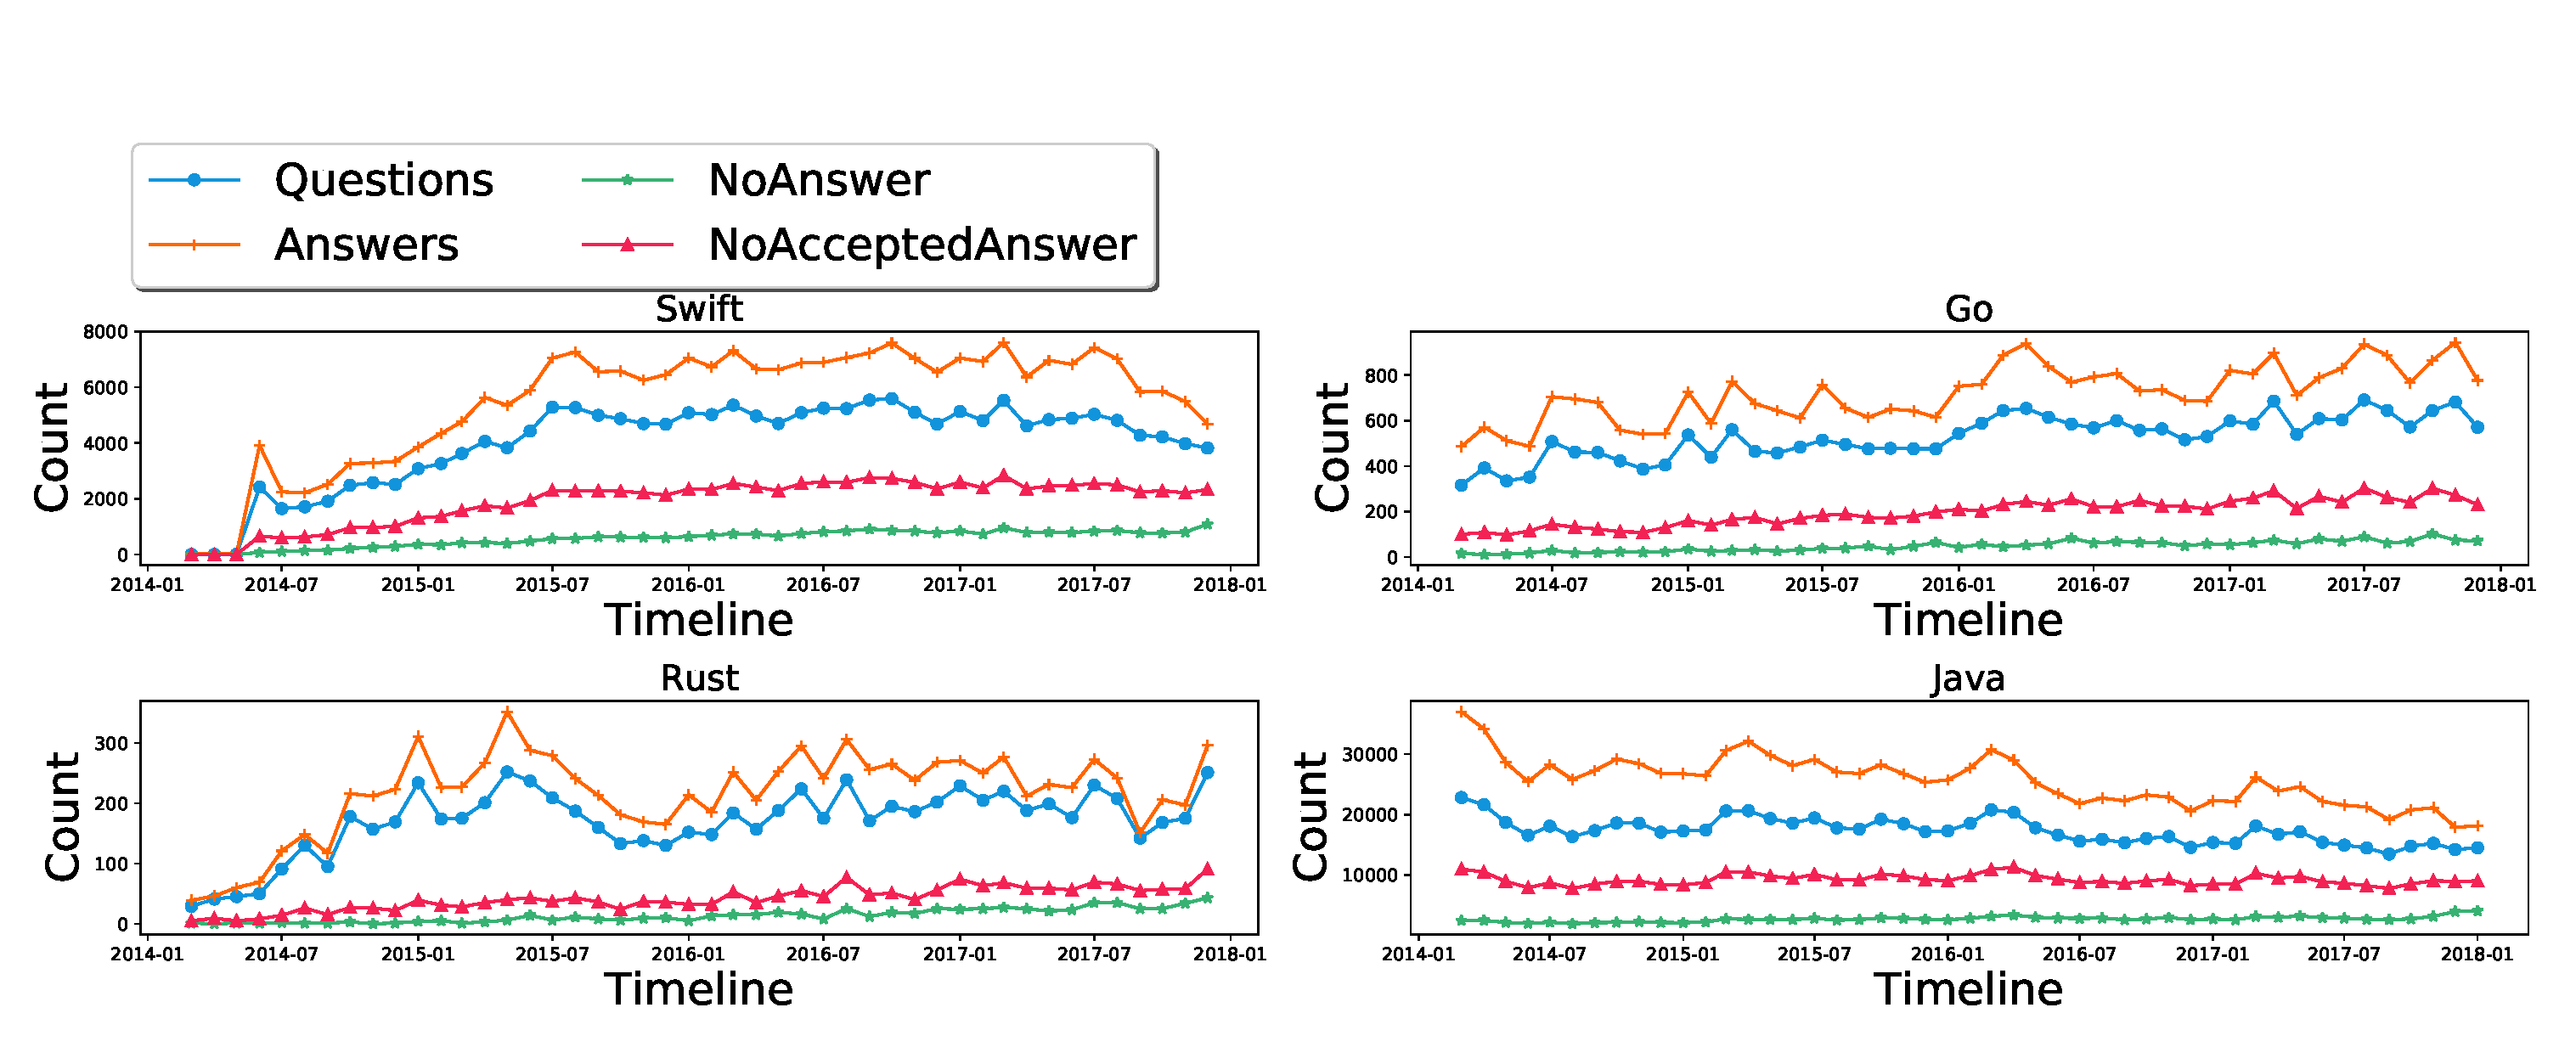
\includegraphics[scale=0.28]{figures/Evolution.eps} 
\caption{Question, No answer, Accepted answer, and No accepted answer count of languages in Stack Overflow}
\label{fig:Evolution of new languages}
\end{figure}

\iffalse
It is prominent in Figure~\ref{fig:Evolution of new languages} that the question count curve of Swift language (Figure~\ref{fig:Attributes of Swift Language}) is much smoother than the other two languages. The reason of smoothness is related to the closed issue ratio. Earlier, we have described the two states of GitHub issue. Based on the two states, we defined the closed issue ratio as,

\begin{equation}
{Closed \quad issue \quad ratio=}
\left[\dfrac{Closed\quad issue}
{Closed\quad issue+Open\quad issue}\right]
\label{eq:Closed Issue Ratio}
\end{equation}

We can say that the closed issue ratio means how much problems have been solved. It can be used as a measure of an active development team. Closed issue ratio one means all problems that were raised in that month were solved. We collected all the issue of the official repositories of new languages and calculated closed issue ratio,

\begin{table}[]
%\centering

\begin{tabular}{|l|l|l|l|}
\hline
 Language& Mean& Variance& Median\\ \hline
 Swift &  0.984  & 0.001 & 0.993 \\ \hline
 Go    &  0.901  & 0.01  & 0.917 \\ \hline
 Rust  &  0.95   & 0.006 & 0.984 \\ \hline

\end{tabular}%

\caption{Statistics of the closed issue ratio of new  languages.}
\label{table:Issue ratio}
\end{table}
From Table~\ref{table:Issue ratio}, we can say Swift has a very active development team with the closed issue ratio close to one. Maybe that is why the question frequency for Swift is smoother than the other two languages.
\fi

Based on the stable date point of new languages presented, we have defined two states for languages (1) Evolving state: the language has just been released, it lacks experts and other resources in Stack Overflow, and (2) Matured State: the language has a stable release with a support community. The details of the stable date point is presented in  in section \ref{RQ1}. Table~\ref{table:States of languages} presents the duration of these states for new languages.
\begin{table}
%\resizebox{\textwidth}{!}{%
\caption{Duration of the evolving and matured state of new languages}
\begin{tabular}{|l|l|l|}
\hline
 Language & Evolving State& Matured State \\ \hline
% Swift & 01/09/14-30/04/16 & 01/05/16-31/12/17  \\ \hline
 Swift & September 2014-October 2016 & November 2016-December 2017  \\ \hline
 Rust & N/A & N/A \\ \hline
 Go & March 2012-June 2015 & July 2015-December 2017 \\ \hline
\end{tabular}%
%}
\label{table:States of languages}
\end{table}
Every answer and question of Stack Overflow is associated with a ``Creation-Date". For each question, we collected all the answers of these questions and by using the ``Creation-Date", we have measured the interval between question and the first answer.
\textcolor{green}{ We must know the distribution  of our data before testing the hypothesis. From the Shapiro-Wilk test\citep{SHAPIRO1965} we found that the distribution of first answer interval distribution does not follow normal distribution. Since non-parametric tests do not assume any distribution, it is widely used in cases where the data does not follow the normal distribution\citep{Mann1947}}. We performed the Mann-Whitney U test which is a non-parametric test to establish the conjecture that it takes more time in the \emph{evolving state} than the \emph{matured state} of their age to have the first answer. The result is presented in Table~\ref{table:Mann-Whitney Test answer interval between states}.


\begin{table}
\centering
\caption{Mann-Whitney U Test result for comparison of the first answer interval between matured and evolving state of new languages}
\begin{tabular}{|l|l|}
\hline
 Language & p value \\ \hline
 Swift & \textless 0.01  \\ \hline
 Rust & Not found \\ \hline
 Go &   \textless 0.01 \\ \hline
\end{tabular}%
\label{table:Mann-Whitney Test answer interval between states}
\end{table}

From the Mann-Whitney test result presented in Table~\ref{table:Mann-Whitney Test answer interval between states}, we have found that only the Swift and Go languages reject the null hypothesis which means that the difference is significant for Swift and Go languages.\\
% According to the release date, Swift is the youngest of these three languages. As a result, when the age is equally divided, it received a small period as evolving state. Even, it may not have reached the matured state yet. On another note, Swift is the direct descendent of Objective-C, and it inherits many libraries and community support from Objective-C. Hence, it may not have an evolving state and started its evolution direct from the matured state. Either of these can be the reason behind the null hypothesis support for Swift.
There may be some differences between topics discussed in the evolving state and the matured state. To test the conjecture, we divided the questions of each language into two states and extracted 10 topics from each state. But the difference was not noticed between the topics. That is because while we are selecting a few topics from large set sub-topics grouped into common programming language topics. To overcome the problem, we extracted 50 topics from each state of each language with their percentage in that stage. If a topic does not appear at both stages, or if their percentage difference is greater than or equal to 2, then we considered that the topic belongs to that stage in which it is most commonly seen. We have tested with various threshold and selected two because otherwise, some topics which are common to all languages irrespective of the stage may appear. Now using this criterion we can identify the topic shift between states of languages.
\begin{enumerate}
\item \textbf{Topics of Swift Language in Evolving State:} During the evolving period, Swift developers mostly talked about language integration and equivalence. Since, in this period, the transition from Objective-C to Swift has just happened, developers were trying to transfer their codebase from Objective-C to Swift. Other popular topics in this state are the use of \emph{alamofire} (a HTTP library) and audio, video controller API of Swift.
\item \textbf{Topics of Swift Language in Matured State:} During the matured state, Swift developers are  mostly concerned about advanced features like ORM, advanced view controllers (segue), and threading. One thing prominent from the data that in matured state Swift developers are asking more questions related to game development such as different type of kits to handle 2D and 3D graphics (sprite kit, scene kit, etc.). The change might be associated with the availability of high-end phones in recent years.\citep{Aleem2016,Gavalas2011}
\item \textbf{Topics of Go Language in Evolving State:} During the evolving state, Go developers discussed compiling issues, compiler path, data types, and type conversion. It seems that developers are trying to understand the syntax and usage of that language. Another common topic in this stage using simple HTTP, TCP, and socket server and encryption technology. As Go is mostly used in the server-side, developers are trying to identify Go's potential by deploying sample project or mimicing old project in the new language.

\item \textbf{Topics of Go Language in Matured State:} In the matured state, Go developers were concerned about HTTP web servers like Gin and  Martini, advanced features like ORM (GORM, GRAIL), and container deployment system Docker, Kubernetes. It is clear that developers are mostly concerned about delivering and deployment system  in this stage.
\end{enumerate}

With the process of evolution, it is expected that the number of unanswered questions will be decreased. To verify this conjecture, we have calculated the unanswered-question ratio for each month. By unanswered question ratio, we mean the ratio of the questions without any answer. We have defined the unanswered question ratio as,

Unanswered question ratio $ = \dfrac{\sum \text{Unanswered questions}}{\sum \text{Questions}}$
\iffalse
\begin{equation}
{\splitdfrac{\quad  \quad Unanswered}{question \quad ratio=}}
\left[\dfrac{\sum Unanswered \quad questions}
{\sum Questions}\right]
\label{eq:Unanswered Question Ratio}
\end{equation}
\fi

The Unanswered question ratio against time is presented in Figure~\ref{fig:Unanswered-question ratio}.
\begin{figure}[htbp]
\centering
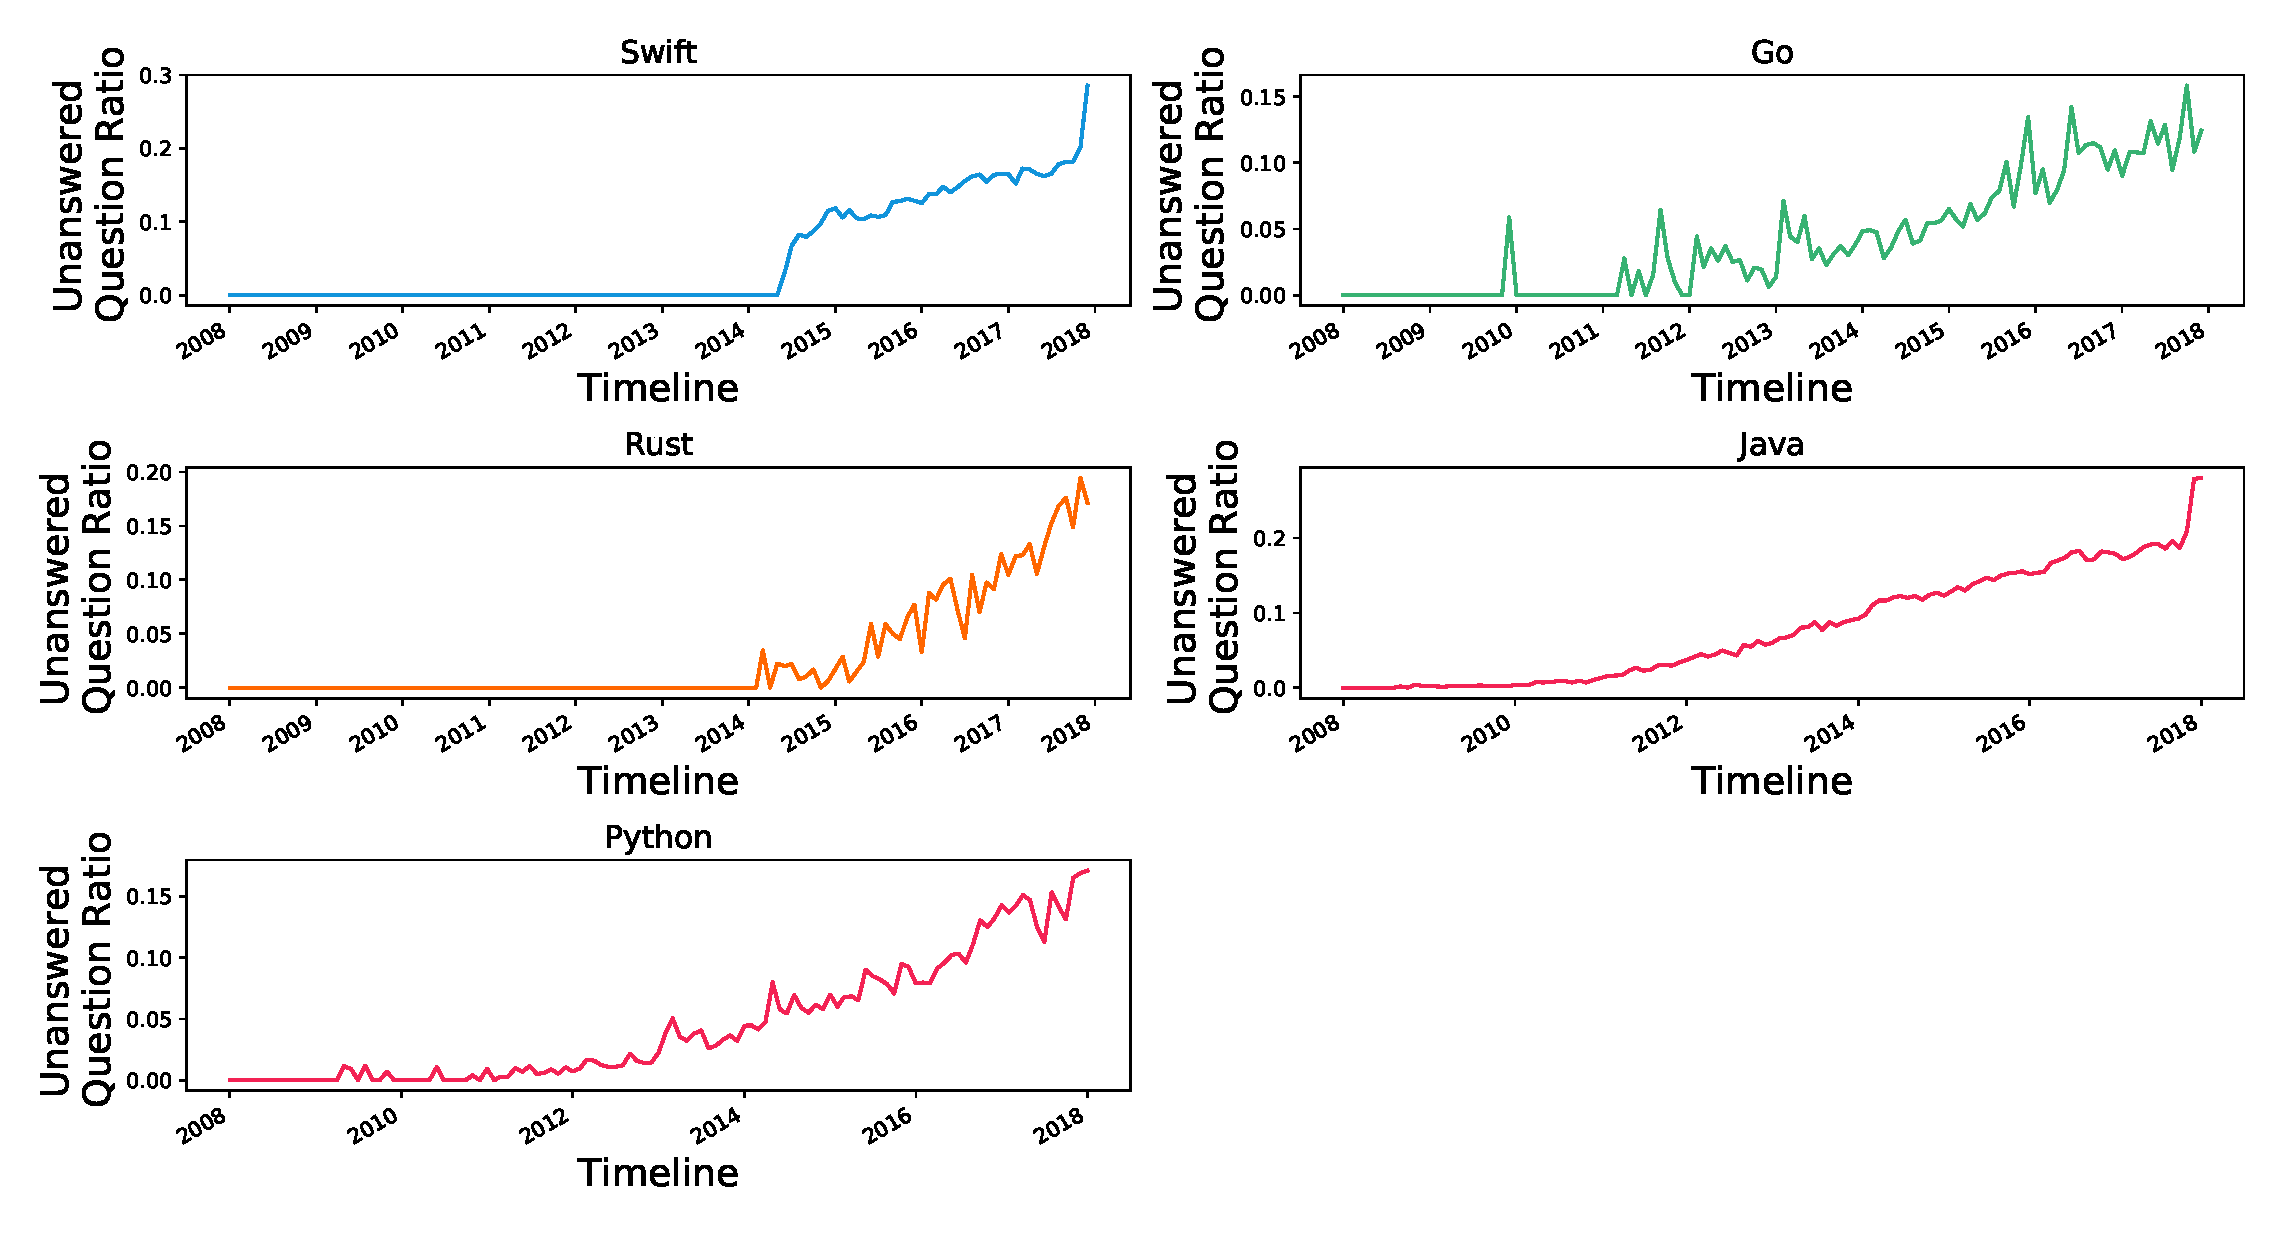
\includegraphics[scale=0.38]{figures/UnansweredQuestionRatio.eps}
\caption{Unanswered-question ratio in Stack Overflow}
\label{fig:Unanswered-question ratio}
\end{figure}


Figure~\ref{fig:Unanswered-question ratio} represents the contrariwise scenery of our assumption. As the day goes by, the unanswered question ratio increases. In one sense, we can say that the answer pattern for new languages and matured languages are the same as in both cases the unanswered question ration increases. However, we can observe two interesting phenomena from these results. First, the change ratio is smoother for matured language while it is notched for new languages except Swift. The reason for the jagged curve may be the absence of active expert developers. Inactive expert developers can change the ratio of the unanswered question by being active for a short time. That is why the curve for Go and Rust are jagged. Being the direct successor of Objective-C, Swift language has avoided this phenomenon. Second, Swift language starts its rise from a certain level which is caused by topic and question inheritance from Objective-C.

To compare growth, we plot the median time to get the first answer and the accepted answer of new languages, one top-tier language (in this case Java), and mid-category language (Python).
\begin{figure}[htbp]
\begin{subfigure}{0.6\textwidth}
\centering
\hspace{-3cm}
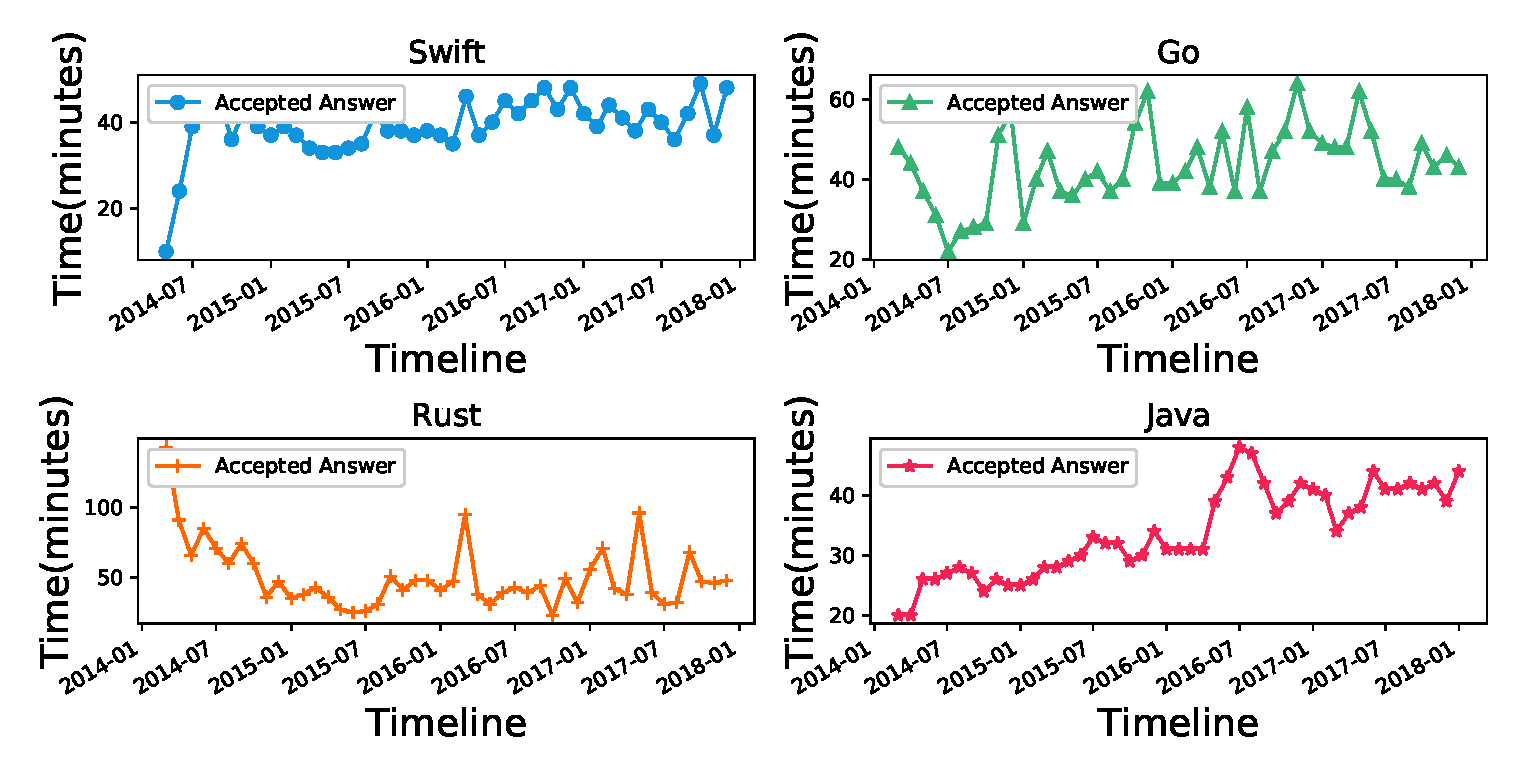
\includegraphics[scale=0.38]{figures/AcceptedAnswerInterval.eps}
\caption{\textbf{Accepted answer}}
\label{fig:Accepted Answer interval}
\end{subfigure}
\begin{subfigure}{0.6\textwidth}
\centering
\hspace{-3cm}
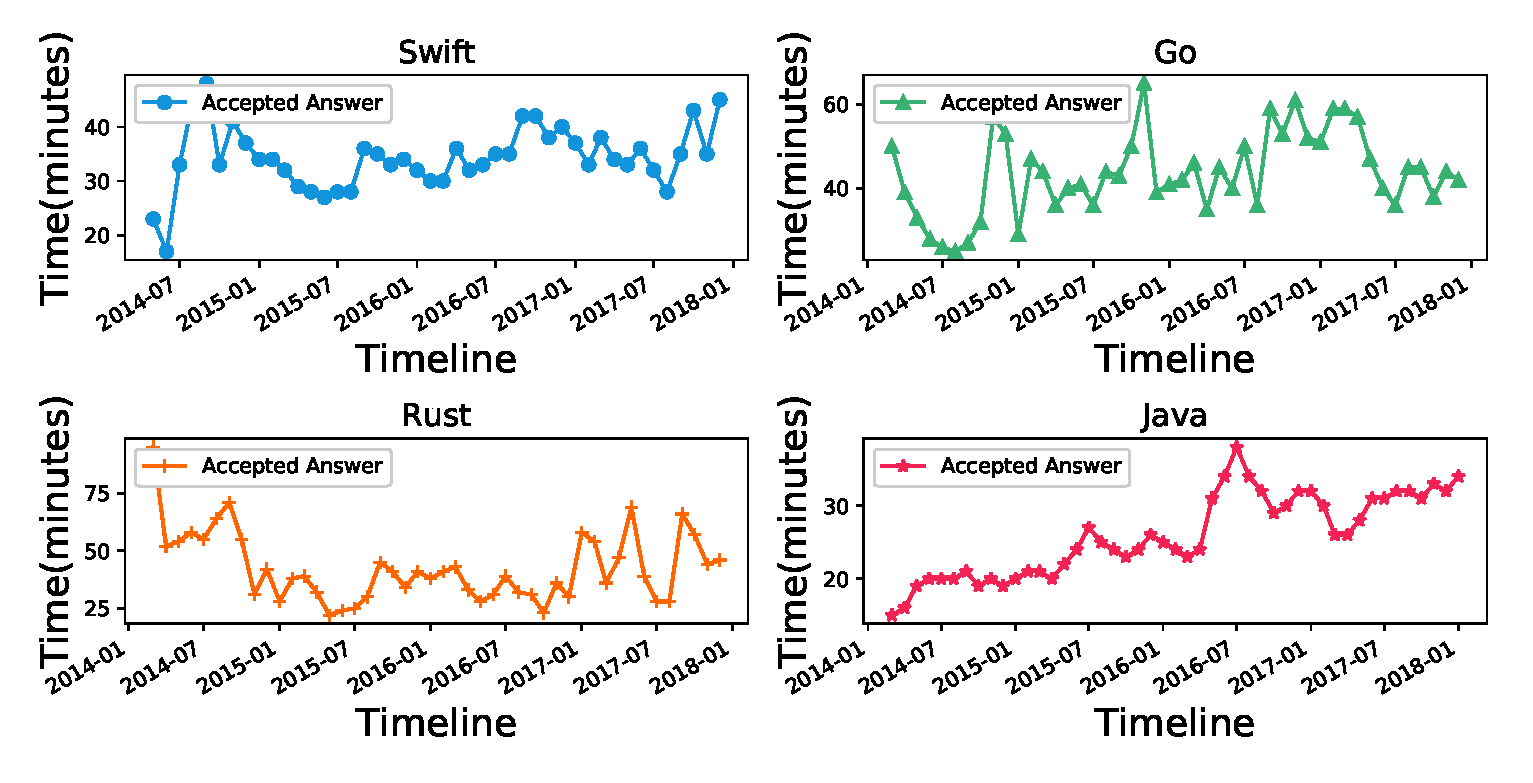
\includegraphics[scale=0.38]{figures/FirstAnswerInterval.eps}
\caption{\textbf{First answer}}
\label{fig:First Answer interval}
\end{subfigure}
\caption{Comparison of median answer interval  of languages in Stack Overflow}
\label{fig:Answer intervals}
\end{figure}
It is assumed that the interval of answers (first and accepted) will be decreased as the language evolves. Figure~\ref{fig:Answer intervals} proves that our assumption is wrong. The answer intervals of Java is increasing in the long run which may be caused by various reason. However, a common reason behind the long answer interval of  stack overflow questions is the inability of that question to attract an expert user to answer that question\citep{Asaduzzaman2013}. However, we can observe steps in the accepted answer interval and the first answer interval of Python and Java. It points out that after a specific time, the answer interval increases. It is common in SO that matured communities often face repeated questions and \emph{hit and run}\citep{DBLP:journals/corr/ChengDL14,SO:decay} problems that cease the necessity of  community collaboration significantly. The increment of answer interval for Python and Java language can be associated with that.
Time to get an accepted answer indirectly represents the growth of developers' expertise. From Figure~\ref{fig:Accepted Answer interval}, it is prominent that Rust has comparatively longer accepted answer interval than the other two new languages. However, it is interesting that this is not true for the first answer interval. Go has longer first answer interval than Rust. Hence, we can say that the accepted answer interval of Rust is longer than Go but Go's first answer interval is longer than Rust. Longer accepted answer interval means the absence of expert developers. Thus, for the Go language, we can claim that Go developers receive the quality answer in the long run, but they have to wait a little longer as active support is absent. That means Stack overflow needs more \emph{active} Go developers and \emph{expert} Rust developers.


\textcolor{green}{To strengthen our claim, we have performed hypothesis testing on accepted answer interval and first answer interval of new languages. To find suitable testing method for hypothesis testing we have performed the Shapiro-Wilk test \citep{SHAPIRO1965}. The Shapiro-Wilk test pointed that the distribution is not normal. Thus we have performed Mann-Whitney U test on first answer interval and accepted answer interval.} The result is presented in Table~\ref{table:accepted-first u value}.
\iffalse
\begin{table}
\centering
%\resizebox{\textwidth}{!}
\caption{Mann-Whitney U test result for the comparison of accepted answer time and first answer time of Go and Rust language}
\label{table:accepted-first u value}
\end{table}
\fi



\begin{table}
\caption{Mann-Whitney U test result for the comparison of accepted answer time and first answer time of Go and Rust language}
\begin{tabular}{|l|c|c|c|}
\hline
\multirow{2}{*}{Test Subject}                                   & \multicolumn{2}{c|}{Language}                                     & \multicolumn{1}{l|}{\multirow{2}{*}{p value}} \\ \cline{2-3}
                                                                & \multicolumn{1}{l|}{Language 1} & \multicolumn{1}{l|}{Language 2} & \multicolumn{1}{l|}{}                         \\ \hline
\multirow{3}{*}{First Answer Interval}                          & Go                              & Swift                           &     0.158                                          \\ \cline{2-4} 
                                                                & Go                              & Rust                            &    \textless 0.01                                           \\ \cline{2-4} 
                                                                & Swift                           & Rust                            &      \textless 0.01                                         \\ \hline
\multicolumn{1}{|c|}{\multirow{3}{*}{Accepted Answer Interval}} & Go                              & Swift                           &        0.389                                       \\ \cline{2-4} 
\multicolumn{1}{|c|}{}                                          & Swift                           & Rust                            &         \textless 0.1                                      \\ \cline{2-4} 
\multicolumn{1}{|c|}{}                                          & Go                           & Rust                            &           \textless 0.01                                    \\ \hline
\end{tabular}

\label{table:accepted-first u value}
\end{table}


From the Table~\ref{table:accepted-first u value}, we can reject the null hypothesis for first answer interval and accepted answer interval of Go-Rust and Swift-Rust pair. It means that the difference between first answer interval and accepted answer interval of Rust-Go and Swift-Rust is statistically significant. It implies that our claim about the first and accepted answer intervals of Go and Rust is true.

\boxtext{\textbf{Finding 7:} In Stack Overflow, it takes significantly higher time to get the first answer in the evolving state than the matured state of a new language.}

\boxtext{\textbf{Finding 8:} In Stack Overflow, we found evidence that Go has comparatively less active community support, and Rust has a small number of expert developers.}
